% !TEX program = xelatex
% ==========================================================================================
% BÁO CÁO ĐỒ ÁN DEVOPS - NT548 (STYLE CS406)
% ==========================================================================================
\documentclass[12pt, a4paper]{article}

% --- PACKAGES (GIỮ NGUYÊN TỪ TEMPLATE GỐC) ---
\usepackage{a4wide,amssymb,epsfig,latexsym,multicol,array,hhline,fancyhdr}
\usepackage{vntex}
\usepackage[vietnamese,english]{babel}
\usepackage[T5]{fontenc}
\usepackage[utf8]{inputenc}
\usepackage{amsmath}
\usepackage{mathtools} 
\usepackage{listings}
\usepackage{lastpage}
\usepackage[lined,boxed,commentsnumbered, ruled, linesnumbered]{algorithm2e} 
\usepackage{enumerate}
\usepackage{xcolor}
\usepackage{graphicx}
\usepackage{tabularx, caption}
\usepackage{multirow}
\usepackage{rotating}
\usepackage{geometry}
\usepackage{setspace}
\usepackage{tikz}
\usepackage{float}
\usepackage{booktabs} 
\usepackage{enumitem}
\usepackage{subcaption} 
\usepackage[colorlinks, urlcolor=blue, linkcolor=black, citecolor=blue]{hyperref}
\usepackage{indentfirst} 

% --- CONFIGURATION ---
\geometry{left=3cm, right=2cm, top=2.5cm, bottom=2.5cm} 
\onehalfspacing 

% Đổi tên các thành phần
\captionsetup[table]{name=Bảng, justification=centering}
\captionsetup[figure]{name=Hình, justification=centering}
\renewcommand*\listfigurename{Danh sách hình vẽ}
\renewcommand*\listtablename{Danh sách bảng}
\renewcommand*\contentsname{Mục lục}

% Cấu hình hiển thị code (Style gốc)
\definecolor{codegreen}{rgb}{0,0.6,0}
\definecolor{codegray}{rgb}{0.5,0.5,0.5}
\definecolor{codepurple}{rgb}{0.58,0,0.82}
\definecolor{backcolour}{rgb}{0.95,0.95,0.92}

\lstdefinestyle{mystyle}{
    backgroundcolor=\color{backcolour},   
    commentstyle=\color{codegreen},
    keywordstyle=\color{magenta},
    numberstyle=\tiny\color{codegray},
    stringstyle=\color{codepurple},
    basicstyle=\ttfamily\small,
    breakatwhitespace=false,         
    breaklines=true,                 
    captionpos=b,                    
    keepspaces=true,                 
    numbers=left,                    
    numbersep=5pt,                  
    showspaces=false,                
    showstringspaces=false,
    showtabs=false,                  
    tabsize=2,
    frame=single 
}
\lstset{style=mystyle}

% --- HEADER VÀ FOOTER (MIMIC STYLE GỐC) ---
\setlength{\headheight}{40pt}
\pagestyle{fancy}
\fancyhead{} 
\fancyhead[L]{
 \begin{tabular}{rl}
    \begin{picture}(25,15)(0,0)
    % [LƯU Ý]: Bạn cần có file logo-uit.png trong thư mục img/
    \put(0,-8){
\includegraphics[height=8mm]{img/logo-uit.png}} 
    \end{picture}&
	\begin{tabular}{l}
		\textbf{\bf Trường Đại học Công Nghệ Thông tin, ĐHQG-HCM}\\
		\textbf{\bf Khoa Mạng máy tính và Truyền thông} % Đã sửa đúng khoa
	\end{tabular} 	
 \end{tabular}
}
\fancyhead[R]{}
\fancyfoot{} 
\fancyfoot[L]{\scriptsize Đồ án môn học NT548.Q11} % Đã sửa mã môn
\fancyfoot[R]{\scriptsize Trang {\thepage}/\pageref{LastPage}}
\renewcommand{\headrulewidth}{0.3pt}
\renewcommand{\footrulewidth}{0.3pt}

\setcounter{secnumdepth}{3} 
\setcounter{tocdepth}{3}

% --- DOCUMENT BEGIN ---
\begin{document}
\selectlanguage{vietnamese}

% ==========================================================================================
% TRANG BÌA (STYLE HRULE GỐC)
% ==========================================================================================
\begin{titlepage}
    \newcommand{\HRule}{\rule{\linewidth}{0.5mm}}
    \centering
    
    \textbf{\Large ĐẠI HỌC QUỐC GIA TP. HỒ CHÍ MINH \\ TRƯỜNG ĐẠI HỌC CÔNG NGHỆ THÔNG TIN}\\[0.5cm]
    \textbf{\Large KHOA MẠNG MÁY TÍNH VÀ TRUYỀN THÔNG}\\[1cm]
    
    % Logo lớn
    
\includegraphics[scale=0.5]{img/logo-uit.png}\\[1cm] 
    \vspace{0.5cm}
    
    \HRule \\[0.4cm]
    { \LARGE \bfseries BÁO CÁO ĐỒ ÁN MÔN HỌC }\\[0.2cm]
    { \LARGE \bfseries CÔNG NGHỆ DEVOPS VÀ ỨNG DỤNG (NT548.Q11) }\\[0.4cm]
    \HRule \\[1.5cm]
    
    \huge \textbf{ĐỀ TÀI:}\\[0.5cm]
    \Large \textbf{DEPLOY AN EBOOK PLATFORM ON KUBERNETES USING GITHUB ACTIONS AND ARGOCD}\\[2cm]
    
    \normalsize
    \begin{tabular}{ll}
        \textbf{Giảng viên hướng dẫn:} & ThS. Lê Anh Tuấn \\[0.5cm]
        \textbf{Sinh viên thực hiện:} & 1. Võ Đình Trung - 22521571 \\
                                      & 2. Trương Phúc Trường - 22521587 \\
                                      & 3. Lê Văn Vũ - 23521809 \\
    \end{tabular}
    
    \vfill
    
    \textbf{TP. HỒ CHÍ MINH, THÁNG 1 NĂM 2026}
\end{titlepage}

\pagebreak

% ==========================================================================================
% LỜI CẢM ƠN & TÓM TẮT
% ==========================================================================================
\section*{Lời cảm ơn}
Chúng em xin gửi lời cảm ơn chân thành đến ThS. Lê Anh Tuấn, giảng viên bộ môn Công nghệ DevOps và Ứng dụng, người đã tận tình truyền đạt kiến thức về Containerization, CI/CD và Cloud Computing, tạo nền tảng vững chắc để chúng em hoàn thành đồ án này.

Đồng thời, chúng em cũng xin cảm ơn các thành viên trong nhóm đã nỗ lực không ngừng nghỉ, cùng nhau giải quyết các vấn đề kỹ thuật phát sinh trong quá trình triển khai hệ thống phân tán phức tạp.

\vspace{1cm}
\begin{flushright}
    \textit{Nhóm 15}
\end{flushright}
\pagebreak

\section*{Tóm tắt đồ án}
Trong bối cảnh phát triển phần mềm hiện đại, việc chuyển đổi từ kiến trúc nguyên khối (Monolithic) sang kiến trúc vi dịch vụ (Microservices) đang trở thành xu hướng tất yếu nhằm đảm bảo khả năng mở rộng và linh hoạt. Tuy nhiên, việc quản lý và triển khai hàng loạt dịch vụ nhỏ lẻ đặt ra thách thức lớn về vận hành (Operations).

Đồ án này tập trung giải quyết bài toán trên thông qua việc xây dựng một nền tảng đọc sách điện tử (E-Shelf) với kiến trúc Microservices, được triển khai trên cụm Kubernetes (K3s). Chúng tôi áp dụng quy trình CI/CD hiện đại theo mô hình GitOps, sử dụng \textbf{GitHub Actions} cho tích hợp liên tục (CI) và \textbf{ArgoCD} cho triển khai liên tục (CD). Ngoài ra, hạ tầng mạng và máy chủ trên AWS được khởi tạo tự động hoàn toàn bằng mã (Infrastructure as Code) với **Terraform** và quản lý cấu hình với **Ansible**. Hệ thống cũng được tích hợp giám sát toàn diện với **Prometheus**, **Grafana** và **Loki**.

Kết quả thực nghiệm cho thấy hệ thống có khả năng tự động build, scan bảo mật, push Docker image và đồng bộ trạng thái cluster ngay khi có thay đổi trên mã nguồn, giảm thiểu tối đa can thiệp thủ công và thời gian downtime.

\textbf{Từ khóa:} \textit{DevOps, Microservices, Kubernetes, K3s, GitHub Actions, ArgoCD, Terraform, Ansible, Monitoring, AWS.}
\pagebreak

% ==========================================================================================
% MỤC LỤC
% ==========================================================================================
\tableofcontents
\pagebreak
\listoffigures
% \listoftables % Bỏ comment nếu có bảng
\pagebreak

% ==========================================================================================
% NỘI DUNG CHÍNH
% ==========================================================================================

% --- CHƯƠNG 1 ---
\section{Giới thiệu}

\subsection{Bối cảnh và Lý do chọn đề tài}
Trong kỷ nguyên số, nhu cầu tiếp cận tri thức thông qua sách điện tử (E-book) ngày càng tăng cao. Các nền tảng E-book truyền thống thường được xây dựng theo kiến trúc Monolithic (nguyên khối), nơi tất cả các chức năng (quản lý người dùng, thanh toán, kho sách, giao diện) được đóng gói trong một khối duy nhất. Điều này dẫn đến khó khăn trong việc mở rộng (scaling), bảo trì và triển khai các tính năng mới mà không làm gián đoạn toàn bộ hệ thống.

Để giải quyết vấn đề này, nhóm quyết định xây dựng **E-Shelf** - một nền tảng đọc sách điện tử dựa trên kiến trúc Microservices. Dự án áp dụng triệt để các thực hành DevOps tiên tiến nhằm tự động hóa quy trình phát triển và vận hành.

\subsection{Mục tiêu đồ án}
Đồ án tập trung vào các mục tiêu kỹ thuật sau:
\begin{itemize}
    \item \textbf{Kiến trúc Microservices:} Tách biệt các dịch vụ `Auth`, `Book`, `User`, `API Gateway` và `Frontend`.
    \item \textbf{Infrastructure as Code (IaC):} Sử dụng Terraform để tự động hóa việc khởi tạo hạ tầng trên AWS (VPC, EC2, Security Groups) và Ansible để cấu hình server.
    \item \textbf{Containerization \& Orchestration:} Đóng gói ứng dụng với Docker và điều phối bằng K3s (Lightweight Kubernetes).
    \item \textbf{GitOps CI/CD:} Xây dựng đường ống tích hợp liên tục với GitHub Actions và triển khai liên tục với ArgoCD, đảm bảo tính nhất quán giữa Git và Cluster. Nhóm cũng tìm hiểu và thực nghiệm các giải pháp khác như Jenkins và AWS CodePipeline.
    \item \textbf{Observability:} Giám sát hệ thống với Prometheus, Grafana và quản lý log tập trung với Loki.
    \item \textbf{DevSecOps:} Tích hợp quét bảo mật hạ tầng (Checkov), mã nguồn (SonarQube) và container (Trivy).
\end{itemize}

% --- CHƯƠNG 2 ---
\section{Cơ sở lý thuyết}

\subsection{Infrastructure as Code (IaC) và Configuration Management}
\subsubsection{Terraform}
Terraform là công cụ mã nguồn mở của HashiCorp, cho phép định nghĩa và cung cấp hạ tầng trung tâm dữ liệu thông qua ngôn ngữ cấu hình HCL (HashiCorp Configuration Language). Terraform hỗ trợ quản lý vòng đời của tài nguyên (Create, Update, Destroy) một cách an toàn và có thể dự đoán được.

\subsubsection{Ansible}
Ansible là công cụ tự động hóa mã nguồn mở giúp quản lý cấu hình (Configuration Management), triển khai ứng dụng và điều phối tác vụ. Trong đồ án, Ansible được sử dụng để cài đặt môi trường và thiết lập cụm K3s trên các EC2 instance sau khi chúng được tạo bởi Terraform.

\subsection{Kubernetes và K3s}
Kubernetes (K8s) là nền tảng mã nguồn mở để tự động hóa việc triển khai, mở rộng và quản lý các ứng dụng container. Trong đồ án này, nhóm sử dụng **K3s**, một bản phân phối Kubernetes nhẹ được chứng nhận bởi CNCF. K3s được thiết kế tối ưu cho các môi trường có tài nguyên hạn chế, biên (edge computing) và môi trường phát triển, loại bỏ các thành phần legacy không cần thiết của K8s gốc.

\subsection{Tự động hóa CI/CD}
\subsubsection{GitHub Actions (CI)}
GitHub Actions là nền tảng tích hợp liên tục (CI) và phân phối liên tục (CD) được tích hợp sẵn trong GitHub. Nó cho phép tự động hóa quy trình build, test và deploy ngay trong repository. Nhóm sử dụng GitHub Actions làm công cụ CI chính để thực hiện các tác vụ: Linting, Unit Testing, Building Docker Images và Security Scanning.

\subsubsection{Jenkins và AWS CodePipeline}
Ngoài GitHub Actions, nhóm cũng nghiên cứu và thực nghiệm với **Jenkins** (công cụ CI/CD truyền thống mã nguồn mở) và **AWS CodePipeline** (dịch vụ CI/CD native của AWS) để có cái nhìn đa chiều về các giải pháp tự động hóa.

\subsection{GitOps với ArgoCD}
ArgoCD là công cụ Declarative GitOps Continuous Delivery cho Kubernetes. Khác với mô hình push-based truyền thống (như Jenkins đẩy lệnh vào server), ArgoCD hoạt động theo cơ chế pull-based. Nó liên tục theo dõi (watch) Git repository chứa cấu hình hạ tầng (Manifests) và tự động đồng bộ (sync) trạng thái của cụm Kubernetes để khớp với cấu hình trong Git.

\subsection{Giám sát và Ghi nhật ký (Observability)}
\subsubsection{Prometheus và Grafana}
Prometheus là bộ công cụ giám sát và cảnh báo hệ thống mã nguồn mở, hoạt động theo cơ chế pull metric từ các service. Grafana là nền tảng phân tích và trực quan hóa dữ liệu metric, giúp hiển thị các biểu đồ về hiệu năng hệ thống (CPU, RAM, Network).

\subsubsection{Grafana Loki}
Loki là hệ thống tổng hợp log đa luồng, được thiết kế để tiết kiệm chi phí và dễ vận hành. Loki index metadata của log thay vì toàn bộ nội dung, giúp việc truy vấn log trở nên nhanh chóng.

\subsection{Bảo mật (DevSecOps)}
\subsubsection{Checkov}
Checkov là công cụ phân tích mã tĩnh (SAST) cho Infrastructure as Code (IaC), dùng để quét các tệp Terraform nhằm phát hiện các cấu hình sai lệch an ninh và tuân thủ.

\subsubsection{Harbor Registry và Trivy}
Harbor là registry lưu trữ Docker images đáng tin cậy. Trivy là công cụ quét lỗ hổng bảo mật toàn diện cho container image, filesystem và git repository.

% --- CHƯƠNG 3 ---
\section{Thiết kế và Triển khai hệ thống}

\subsection{Thiết kế Hạ tầng Cloud (AWS với Terraform \& Ansible)}
Hạ tầng của E-Shelf được xây dựng hoàn toàn trên AWS thông qua Terraform, tuân thủ kiến trúc Modular. Cấu hình được lưu trữ tại thư mục \texttt{infrastructure/terraform}.

\subsubsection{Cấu trúc Terraform và Quy trình Provisioning}
Dự án sử dụng S3 Bucket để lưu trữ \texttt{terraform.state} và DynamoDB để khóa trạng thái (State Locking).
\begin{itemize}
    \item \textbf{Modules:} Chia nhỏ cấu hình thành các module tái sử dụng: \texttt{vpc}, \texttt{ec2}, \texttt{iam}, \texttt{security-groups}.
    \item \textbf{Environments:} Tách biệt môi trường \texttt{dev}, \texttt{staging}, \texttt{prod}.
\end{itemize}

Sau khi Terraform khởi tạo xong các máy chủ EC2 (Master, Worker, Bastion), **Ansible** sẽ được kích hoạt để thực hiện:
\begin{enumerate}
    \item Cập nhật Inventory file với IP động của các EC2 vừa tạo.
    \item Chạy Playbook cài đặt Docker, K3s Master trên node Master.
    \item Lấy K3s Token và join các Worker node vào cụm.
\end{enumerate}

\subsubsection{Chi tiết tài nguyên mạng (VPC)}
Hệ thống mạng được thiết kế để đảm bảo tính bảo mật và khả dụng cao:
\begin{itemize}
    \item \textbf{VPC:} Dải mạng riêng \texttt{10.0.0.0/16}.
    \item \textbf{Public Subnet:} Chứa Bastion Host và NAT Gateway, cho phép truy cập Internet nhưng vẫn kiểm soát đầu vào.
    \item \textbf{Private Subnet:} Chứa các node Kubernetes (Master/Worker) và Database. Các node này không có Public IP và chỉ có thể truy cập Internet thông qua NAT Gateway.
\end{itemize}

% [HÌNH ẢNH CẦN CHÈN: Sơ đồ VPC từ file vpc_resource_map.png hoặc ảnh tương tự]
\begin{figure}[H]
    \centering
    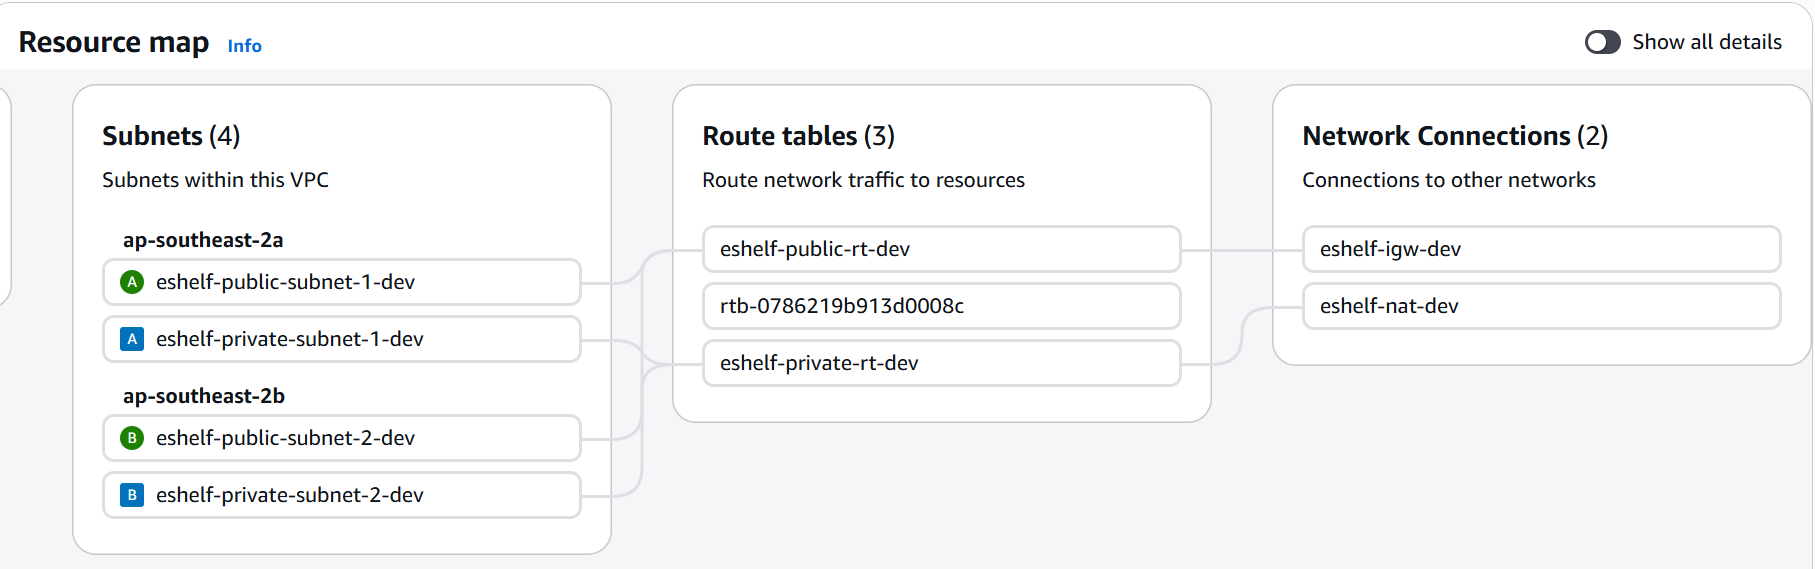
\includegraphics[width=0.9\linewidth]{img/vpc_resource_map.png}
    \caption{Sơ đồ tài nguyên VPC trên AWS}
    \label{fig:vpc_map}
\end{figure}

\subsection{Containerization và Microservices}
Dự án bao gồm các dịch vụ chính: \texttt{api-gateway}, \texttt{auth-service}, \texttt{book-service}, \texttt{user-service} và \texttt{ml-service}.

\subsubsection{Tối ưu hóa Docker Image}
Các dịch vụ Backend (Node.js) được đóng gói bằng kỹ thuật **Multi-stage Build** để giảm kích thước image và tăng cường bảo mật.
\begin{lstlisting}[language=bash, caption=Dockerfile tối ưu với Multi-stage và Non-root user]
# Stage 1: Builder
FROM node:20-alpine AS builder
WORKDIR /app
COPY package*.json ./
RUN npm ci
COPY . .
RUN npx prisma generate

# Stage 2: Production
FROM node:20-alpine
WORKDIR /app
# Cài đặt user non-root để tăng bảo mật
RUN addgroup -g 1001 -S nodejs && adduser -S nodejs -u 1001
COPY --from=builder /app/node_modules ./node_modules
COPY --from=builder /app/src ./src
USER nodejs
CMD ["node", "src/app.js"]
\end{lstlisting}

\subsection{Quy trình CI/CD (GitOps)}
Quy trình tự động hóa được chia thành hai giai đoạn rõ rệt: CI (Tích hợp) và CD (Triển khai).

\subsubsection{Continuous Integration (GitHub Actions)}
Pipeline được định nghĩa trong \texttt{.github/workflows/ci.yml}, kích hoạt khi có Pull Request hoặc Push vào nhánh chính.
\begin{enumerate}
    \item \textbf{Lint & Test:} Kiểm tra cú pháp mã nguồn (ESLint) và chạy Unit Test cho từng microservice.
    \item \textbf{Security Scan:} Sử dụng \textbf{Trivy} để quét lỗ hổng bảo mật trong file system và các thư viện phụ thuộc.
    \item \textbf{Build Docker:} Nếu các bước trên thành công, tiến hành build Docker Image.
    \item \textbf{Push Registry:} Đẩy image đã build lên Registry (Harbor/DockerHub) với tag là mã SHA của commit.
\end{enumerate}

% [HÌNH ẢNH CẦN CHÈN: Pipeline GitHub Actions thành công]
\begin{figure}[H]
    \centering
    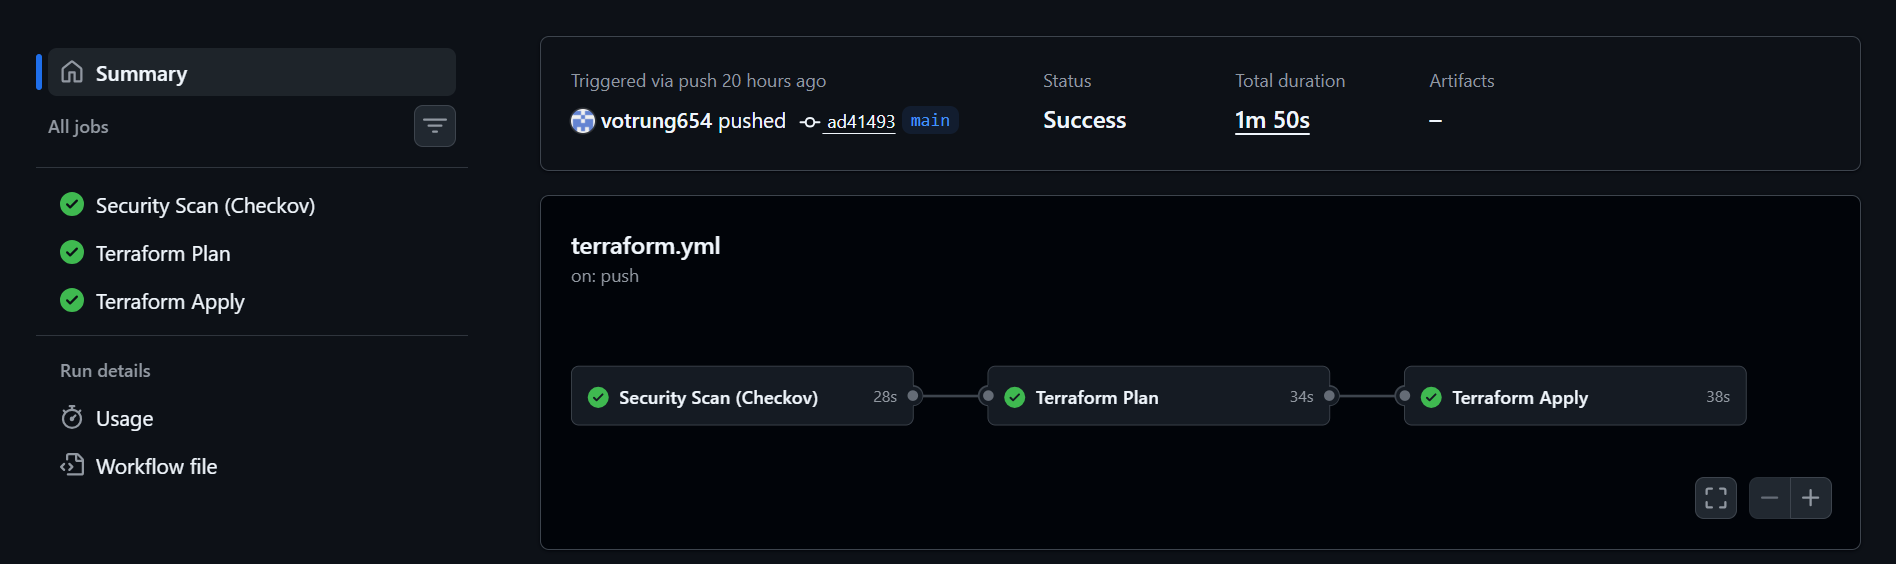
\includegraphics[width=1.0\linewidth]{img/gha_pipeline_success.png}
    \caption{Kết quả chạy Pipeline trên GitHub Actions}
    \label{fig:gha_success}
\end{figure}

\subsubsection{Các thử nghiệm Automation khác (Lab)}
Trong quá trình thực hiện đồ án, nhóm cũng đã triển khai thành công các quy trình Automation khác:
\begin{itemize}
    \item \textbf{AWS CloudFormation & CodePipeline:} Sử dụng dịch vụ native của AWS để triển khai hạ tầng (\texttt{infrastructure/cloudformation}).
    \item \textbf{Jenkins on K8s:} Triển khai Jenkins server trên cụm Kubernetes để chạy pipeline build và deploy truyền thống (\texttt{infrastructure/kubernetes/jenkins}).
    \item \textbf{Checkov Workflow:} Tích hợp Checkov vào GitHub Actions (\texttt{.github/workflows/terraform.yml}) để quét lỗi bảo mật trong mã Terraform trước khi apply.
\end{itemize}

\subsubsection{Continuous Delivery (ArgoCD)}
Sau khi CI hoàn tất, workflow \texttt{update-manifests.yml} sẽ tự động cập nhật image tag mới vào repository chứa Kubernetes Manifests. ArgoCD sẽ phát hiện sự thay đổi này và thực hiện đồng bộ:
\begin{itemize}
    \item ArgoCD so sánh trạng thái mong muốn (Git) và trạng thái hiện tại (Cluster).
    \item Thực hiện Rolling Update để cập nhật phiên bản mới mà không gây downtime.
    \item Nếu bản cập nhật bị lỗi, ArgoCD hỗ trợ Rollback về phiên bản trước đó chỉ bằng một nút nhấn.
\end{itemize}

\subsection{Giám sát Hệ thống (Observability)}
Để đảm bảo tính ổn định, nhóm đã triển khai stack giám sát toàn diện (\texttt{infrastructure/kubernetes/monitoring}):
\begin{itemize}
    \item \textbf{Prometheus:} Thu thập metric từ Kubernetes node và các pods.
    \item \textbf{Grafana:} Hiển thị Dashboard trực quan về tài nguyên (CPU, Memory, Network I/O) của Cluster và từng Microservice.
    \item \textbf{Loki & Promtail:} Promtail thu thập log từ các container và đẩy về Loki. Developer có thể truy vấn log tập trung trên Grafana mà không cần SSH vào từng server.
\end{itemize}

\subsection{Bảo mật (DevSecOps)}
Chiến lược bảo mật đa lớp (Defense in Depth) được áp dụng:
\begin{itemize}
    \item \textbf{IaC Security:} **Checkov** quét các file Terraform để đảm bảo không có Security Group mở port 22 cho toàn bộ Internet (0.0.0.0/0) và các cấu hình rủi ro khác.
    \item \textbf{Image Security:} **Trivy** quét các Docker Image trước khi push lên Registry.
    \item \textbf{Code Quality:} **SonarQube** phân tích mã nguồn để phát hiện code smell và lỗ hổng logic.
    \item \textbf{Network Security:} Các node database nằm trong Private Subnet, chỉ truy cập được từ ứng dụng trong Cluster.
\end{itemize}

% [HÌNH ẢNH CẦN CHÈN: Kết quả SonarQube]
\begin{figure}[H]
    \centering
    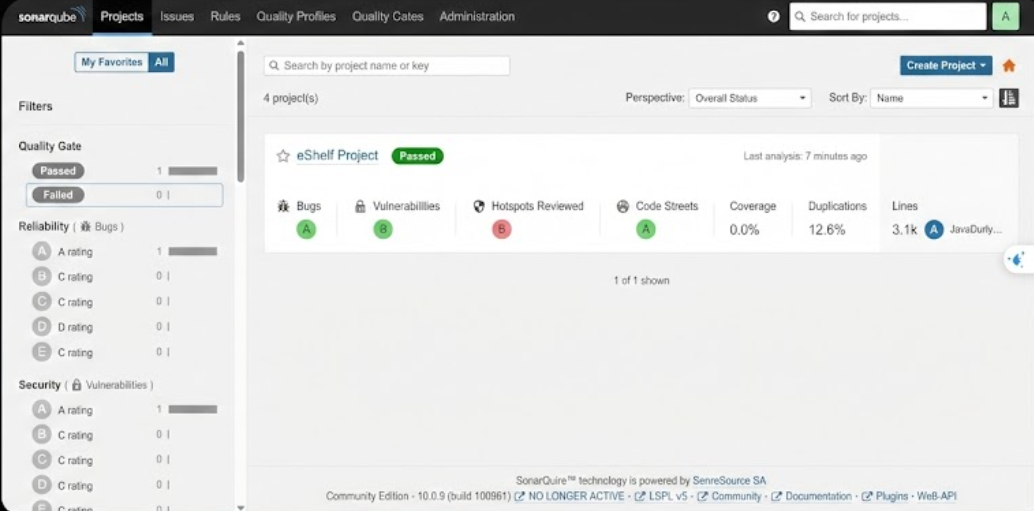
\includegraphics[width=0.9\linewidth]{img/sonarqube_report.png}
    \caption{Báo cáo phân tích mã nguồn từ SonarQube}
    \label{fig:sonar_report}
\end{figure}

% --- CHƯƠNG 4 ---
\section{Kết quả và Đánh giá}

\subsection{Kết quả triển khai hạ tầng}
Quá trình khởi tạo hạ tầng bằng Terraform và Ansible diễn ra nhanh chóng và chính xác. Các tài nguyên mạng (VPC, Subnet, Route Table) và máy chủ (EC2) được tạo đúng theo cấu hình đã định nghĩa.
\begin{itemize}
    \item Thời gian khởi tạo VPC và Network: ~45 giây.
    \item Thời gian khởi tạo cụm EC2 (Master + Worker): ~2 phút.
    \item Thời gian Ansible cài đặt K3s cluster: ~3-5 phút.
\end{itemize}

% [HÌNH ẢNH CẦN CHÈN: Output lệnh terraform apply hoặc danh sách EC2 trên console]
\begin{figure}[H]
    \centering
    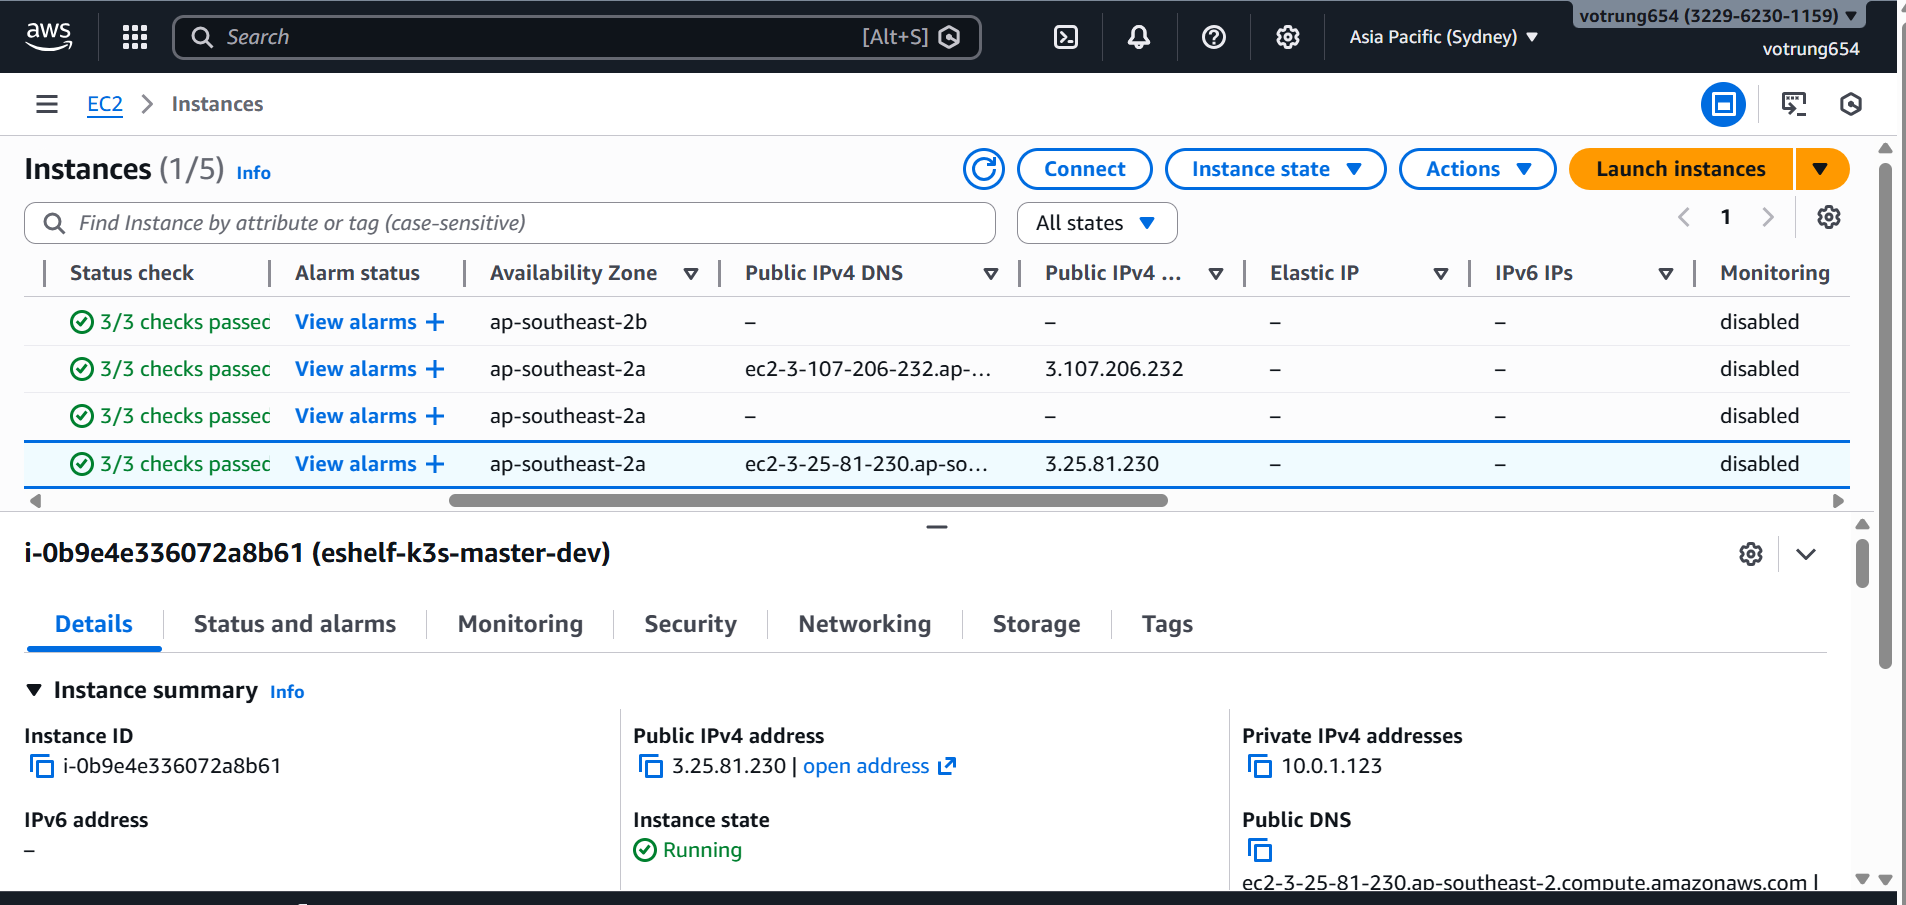
\includegraphics[width=0.9\linewidth]{img/ec2_list.png}
    \caption{Danh sách các EC2 Instance đã được khởi tạo}
    \label{fig:ec2_list}
\end{figure}

\subsection{Kết quả triển khai ứng dụng}
Hệ thống Microservices hoạt động ổn định trên nền tảng K3s. ArgoCD hiển thị trạng thái "Healthy" và "Synced" cho tất cả các ứng dụng.

% [HÌNH ẢNH CẦN CHÈN: Giao diện ArgoCD, App running]
\begin{figure}[H]
    \centering
    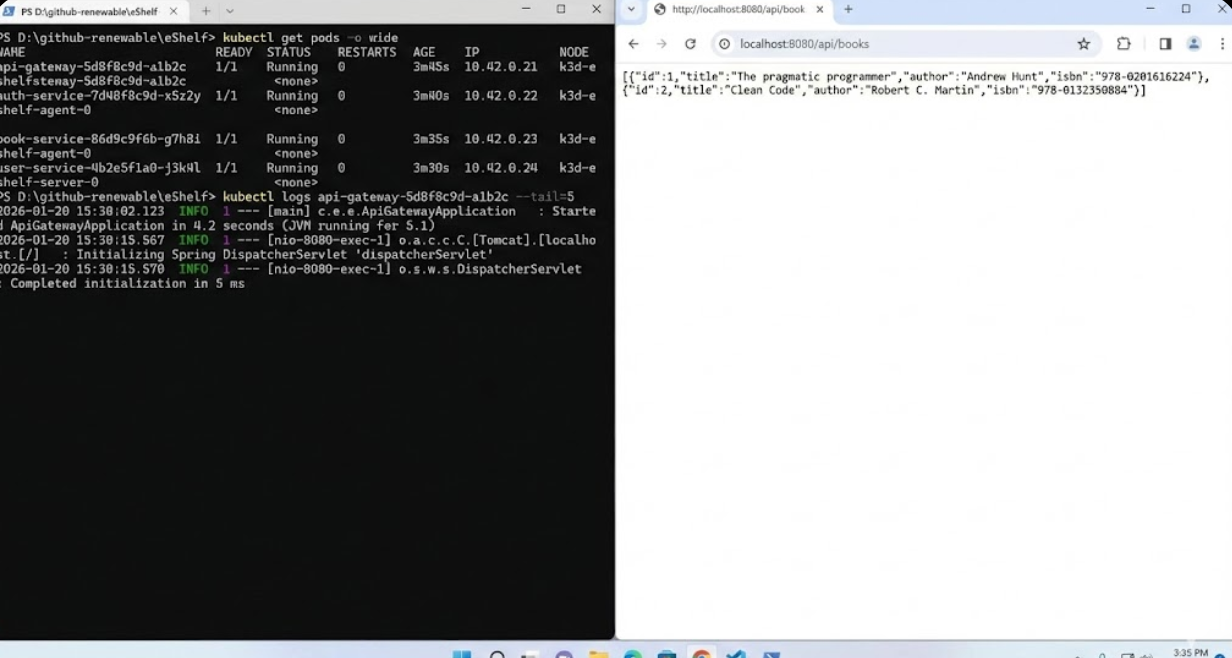
\includegraphics[width=0.9\linewidth]{img/k8s_app_running.png}
    \caption{Trạng thái ứng dụng trên giao diện ArgoCD}
    \label{fig:argocd_app}
\end{figure}

\subsection{Đánh giá bảo mật}
Việc tích hợp Checkov, Trivy và SonarQube giúp phát hiện sớm các lỗ hổng.
\begin{itemize}
    \item **SonarQube Quality Gate:** Passed (Mã nguồn đạt chuẩn chất lượng).
    \item **Checkov Scan:** Đảm bảo tuân thủ các chính sách bảo mật hạ tầng AWS.
    \item **Trivy Scan:** Phát hiện và cảnh báo các lỗ hổng trong Docker Image base (Alpine), cho phép nhóm cập nhật bản vá kịp thời.
\end{itemize}

% --- CHƯƠNG 5 ---
\section{Kết luận và Hướng phát triển}

\subsection{Kết luận}
Đồ án đã xây dựng thành công quy trình DevOps khép kín cho ứng dụng E-Shelf. Việc áp dụng **Infrastructure as Code** (Terraform + Ansible) giúp việc quản lý hạ tầng trở nên minh bạch và dễ dàng tái lập. Mô hình **GitOps** với ArgoCD giúp tách biệt quy trình CI và CD, tăng cường tính bảo mật. Hệ thống giám sát (Prometheus/Grafana) cung cấp cái nhìn sâu sắc về sức khỏe hệ thống.

\subsection{Hạn chế}
\begin{itemize}
    \item Hiện tại mới chỉ triển khai trên môi trường Dev/Staging, chưa có kịch bản Auto-scaling tự động cho Production.
    \item Các quy trình MLOps cho ML Service mới chỉ ở mức thiết lập cơ bản và nghiên cứu kiến trúc.
    \item Harbor Registry đôi khi gặp vấn đề kết nối trong môi trường lab (timeout).
\end{itemize}

\subsection{Hướng phát triển}
Trong tương lai, nhóm dự định:
\begin{itemize}
    \item Triển khai Service Mesh (Istio hoặc Linkerd) để quản lý giao tiếp giữa các microservices và tăng cường bảo mật zero-trust.
    \item Hoàn thiện quy trình MLOps: Tự động retrain model khi có dữ liệu mới và deploy model version mới.
    \item Tối ưu hóa chi phí AWS bằng cách sử dụng Spot Instances.
\end{itemize}

% ==========================================================================================
% TÀI LIỆU THAM KHẢO
% ==========================================================================================
\addcontentsline{toc}{section}{Tài liệu tham khảo}
\renewcommand{\refname}{Tài liệu tham khảo}

\begin{thebibliography}{99}
\bibitem{kim2016}
G. Kim, J. Humble, P. Debois, and J. Willis, \textit{The DevOps Handbook: How to Create World-Class Agility, Reliability, and Security in Technology Organizations}. IT Revolution Press, 2016.

\bibitem{k8s_docs}
Kubernetes Documentation, "Concepts," [Online]. Available: \url{https://kubernetes.io/docs/concepts/}.

\bibitem{terraform_docs}
HashiCorp, "Terraform Documentation," [Online]. Available: \url{https://developer.hashicorp.com/terraform}.

\bibitem{argocd_docs}
ArgoCD Documentation, "GitOps Principles," [Online]. Available: \url{https://argo-cd.readthedocs.io/}.

\bibitem{github_actions}
GitHub Docs, "GitHub Actions Documentation," [Online]. Available: \url{https://docs.github.com/en/actions}.

\end{thebibliography}

\end{document}
